\title{バージョン管理システムチュートリアル}

\begin{document}

\lstset{language={sh},showspaces=false,rulecolor=\color[cmyk]{0, 0.29,0.84,0}}

\begin{frame}
  \titlepage
\end{frame}

\section*{Outline}
\begin{frame}
  \tableofcontents
\end{frame}

\section{チュートリアルの概要}

\begin{frame}{VCSチュートリアル スタッフ}
  \begin{itemize}
  \item 講師
    \begin{itemize}
    \item 藤堂眞治 (東大物性研) \ \href{mailto:wistaria@issp.u-tokyo.ac.jp}{wistaria@issp.u-tokyo.ac.jp}
    \item 五十嵐 亮 (東大物性研) \ \href{mailto:rigarash@issp.u-tokyo.ac.jp}{rigarash@issp.u-tokyo.ac.jp}
    \item 松尾春彦 (RIST) \ \href{mailto:halm@rist.or.jp}{halm@rist.or.jp}
    \item 本山裕一 (東大院工) \ \href{mailto:yomichi@looper.t.u-tokyo.ac.jp}{yomichi@looper.t.u-tokyo.ac.jp}
    \end{itemize}
  \item 主催
    \begin{itemize}
    \item CMSI: 計算物質科学イニシアティブ \url{http://cms-initiative.jp/}
    \end{itemize}
  \item 共催
    \begin{itemize}
    \item RIST: 一般財団法人 高度情報科学技術研究機構 \url{http://www.rist.or.jp/}
    \end{itemize}
  \end{itemize}
\end{frame}

\begin{frame}
  \frametitle{チュートリアルの流れ}
  \begin{itemize}
    %\setlength{\itemsep}{1em}
  \item 準備作業
  \item バージョン管理システムとは? (講義 \& 実習)
  \item gitの基礎 (講義 \& 実習)
  \item ブランチとマージ (講義 \& 実習)
  \item リモートリポジトリとの連携 (講義 \& 実習)
  \item githubを用いたオープンソース・ソフトウェアの開発・公開 (講義 \& 実習)
  \item MateriAppsとMateriApps Liveの紹介
  \item (optional) A successful Git branching model (講義)
  \item (optional) Gitをボトムアップから理解する (講義)
  \end{itemize}
\end{frame}

\section{準備作業}

\begin{frame}
  \frametitle{ネットワーク設定}
  \begin{itemize}
    %\setlength{\itemsep}{1em}
  \item LAN接続 (無線 or 有線)
  \item 実習用ワークステーションのアカウント登録
  \item github アカウント登録 (まだアカウントを持っていない人のみ)
    \begin{itemize}
    \item \url{https://github.com} にアクセス
    \item ``Sign up for GitHub''をクリック、必要事項を記入した後、``Create an account''
    \item SSH公開鍵の登録 (``Account settings'' $\Rightarrow$ ``SSH Keys'')
    \end{itemize} 
  \item sourceforge アカウント登録 (まだアカウントを持っていない人のみ)
    \begin{itemize}
    \item \url{http://sourceforge.net/} にアクセス
    \item 右上の``Join''をクリック、必要事項を記入して``Register''
    \end{itemize} 
  \end{itemize}
\end{frame}

\begin{frame}[t,fragile]
  \frametitle{PCへのgitクライアントのインストール}
  \begin{itemize}
    %\setlength{\itemsep}{1em}
  \item Windows \& Mac OS X
    \begin{itemize}
      \item \url{http://git-scm.com/downloads}からインストーラーをダウンロード
      \item Mac の場合は MacPorts からインストールすることも可
\begin{lstlisting}
$ sudo port install git
\end{lstlisting}
    \end{itemize}
  \item Linux
    \begin{itemize}
      \item Redhat系
\begin{lstlisting}
$ sudo yum install git
\end{lstlisting}
      \item Debian系
\begin{lstlisting}
$ sudo apt-get install git
\end{lstlisting}
    \end{itemize}
  \end{itemize}
\end{frame}

\section{バージョン管理システムの概要}

\begin{frame}
  \frametitle{diff と patch によるバージョン管理}
  \begin{itemize}
    \setlength{\itemsep}{1em}
  \item diff: 2つのテキストファイルの差分を出力するコマンド
    \begin{itemize}
    \item ファイル全体を保存するよりコンパクト
    \item 変更点を確認しやすい
    \end{itemize}
  \item patch: diff コマンドが生成した差分をファイルに適用するユーティリティー
    \begin{itemize}
    \item もとのファイルと差分から変更後のファイルを生成できる
    \end{itemize}
  \end{itemize}
\end{frame}

\begin{frame}[t,fragile]
  \frametitle{実習: diff \& patch (1)}
  \begin{itemize}
    %\setlength{\itemsep}{1em}
  \item 単一ファイルの例
\begin{lstlisting}
$ cp /home/hands-on/vcs/diff/prologue.txt prologue.txt
$ cp prologue.txt prologue-orig.txt
$ vi prologue.txt  # prologue.txt を編集

$ diff -u prologue-orig.txt prologue.txt > prologue.diff
$ less prologue.diff  # prologue.diffの中身を見てみる
  
$ cp /home/hands-on/vcs/diff/prologue.txt prologue.txt
$ patch < prologue.diff
$ less prologue.txt  # prologue.txtの中身を確認
\end{lstlisting}
  \end{itemize}
\end{frame}

\begin{frame}[t,fragile]
  \frametitle{実習: diff \& patch (2)}
  \begin{itemize}
    %\setlength{\itemsep}{1em}
  \item ディレクトリ全体を扱う例
\begin{lstlisting}
$ cp -r /home/hands-on/vcs/diff shake
$ cp -r shake shake.orig
# shakeの中のファイルを編集(ファイルの削除や追加も可)

$ diff -urN shake.orig shake > shake.diff
$ less shake.diff   # shake.diffの中身を見てみる

$ rm -rf shake
$ cp -r /home/hands-on/vcs/diff shake
$ patch -p0 < shake.diff
# shakeの中身を確認
\end{lstlisting}
  \item diff と patch で差分の管理は可能になるが、履歴は別に管理してお
    かなければならない
  \end{itemize}
\end{frame}

\begin{frame}
  \frametitle{バージョン管理システムとは?}
  \begin{columns}[T]
    \begin{column}{.7\textwidth}
      \begin{itemize}
        \setlength{\itemsep}{1em}
      \item ファイルの履歴をデータベース(リポジトリ)で一括管理するシス
        テム
      \item もともとはプログラムのソースコードのためのシステム
        \begin{itemize}
        \item それ以外のファイル(例えば \LaTeX ファイル)管理にも使える
        \end{itemize}
      \item 一人で使っても複数人で使っても超便利
        \begin{itemize}
        \item 超優秀な秘書のようなもの
        \end{itemize}
      \end{itemize}
    \end{column}
    \begin{column}{.25\textwidth}
      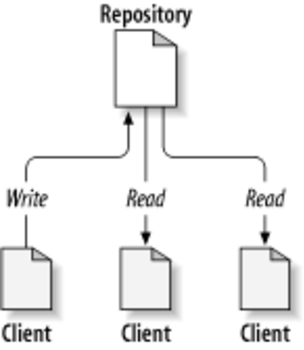
\includegraphics[width=\textwidth]{ch02dia1.pdf}
    \end{column}
  \end{columns}
\end{frame}

\begin{frame}
  \frametitle{なぜバージョン管理システムが必要なのか?}
  \begin{columns}[T]
    \begin{column}{.7\textwidth}
      \begin{itemize}
        \setlength{\itemsep}{1em}
      \item 作業者 and/or 作業場所が複数になると、ファイル名や手書きのログファイルによるバージョン管理はすぐに破綻する
        \begin{itemize}
        \item ネットワーク経由でファイルを check out/check in
        \item 更新毎に一意なバージョン番号 (リビジョン) を付与
        \item 任意のバージョン間の比較が容易
        \item バックアップの代わりにも
        \end{itemize}
      \item 複数箇所から同時に更新した場合に衝突を回避するしくみを備えている
      \item ブランチ・マージ・タグ付けなどが可能
      \end{itemize}
    \end{column}
    \begin{column}{.25\textwidth}
      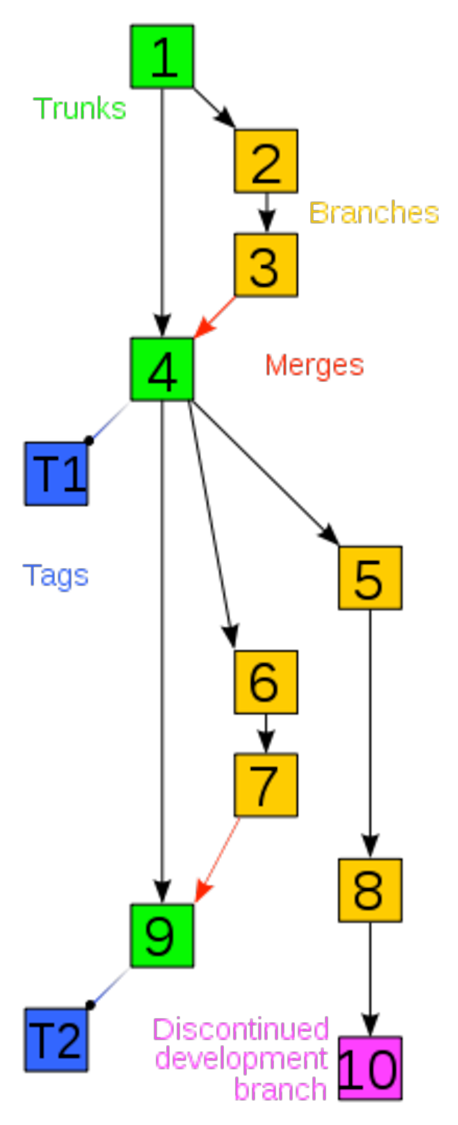
\includegraphics[width=.7\textwidth]{220px-Revision_controlled_project_visualization-2010-24-02.pdf}
    \end{column}
  \end{columns}
\end{frame}

\begin{frame}
  \frametitle{ありがちなパターン}
  \begin{center}
    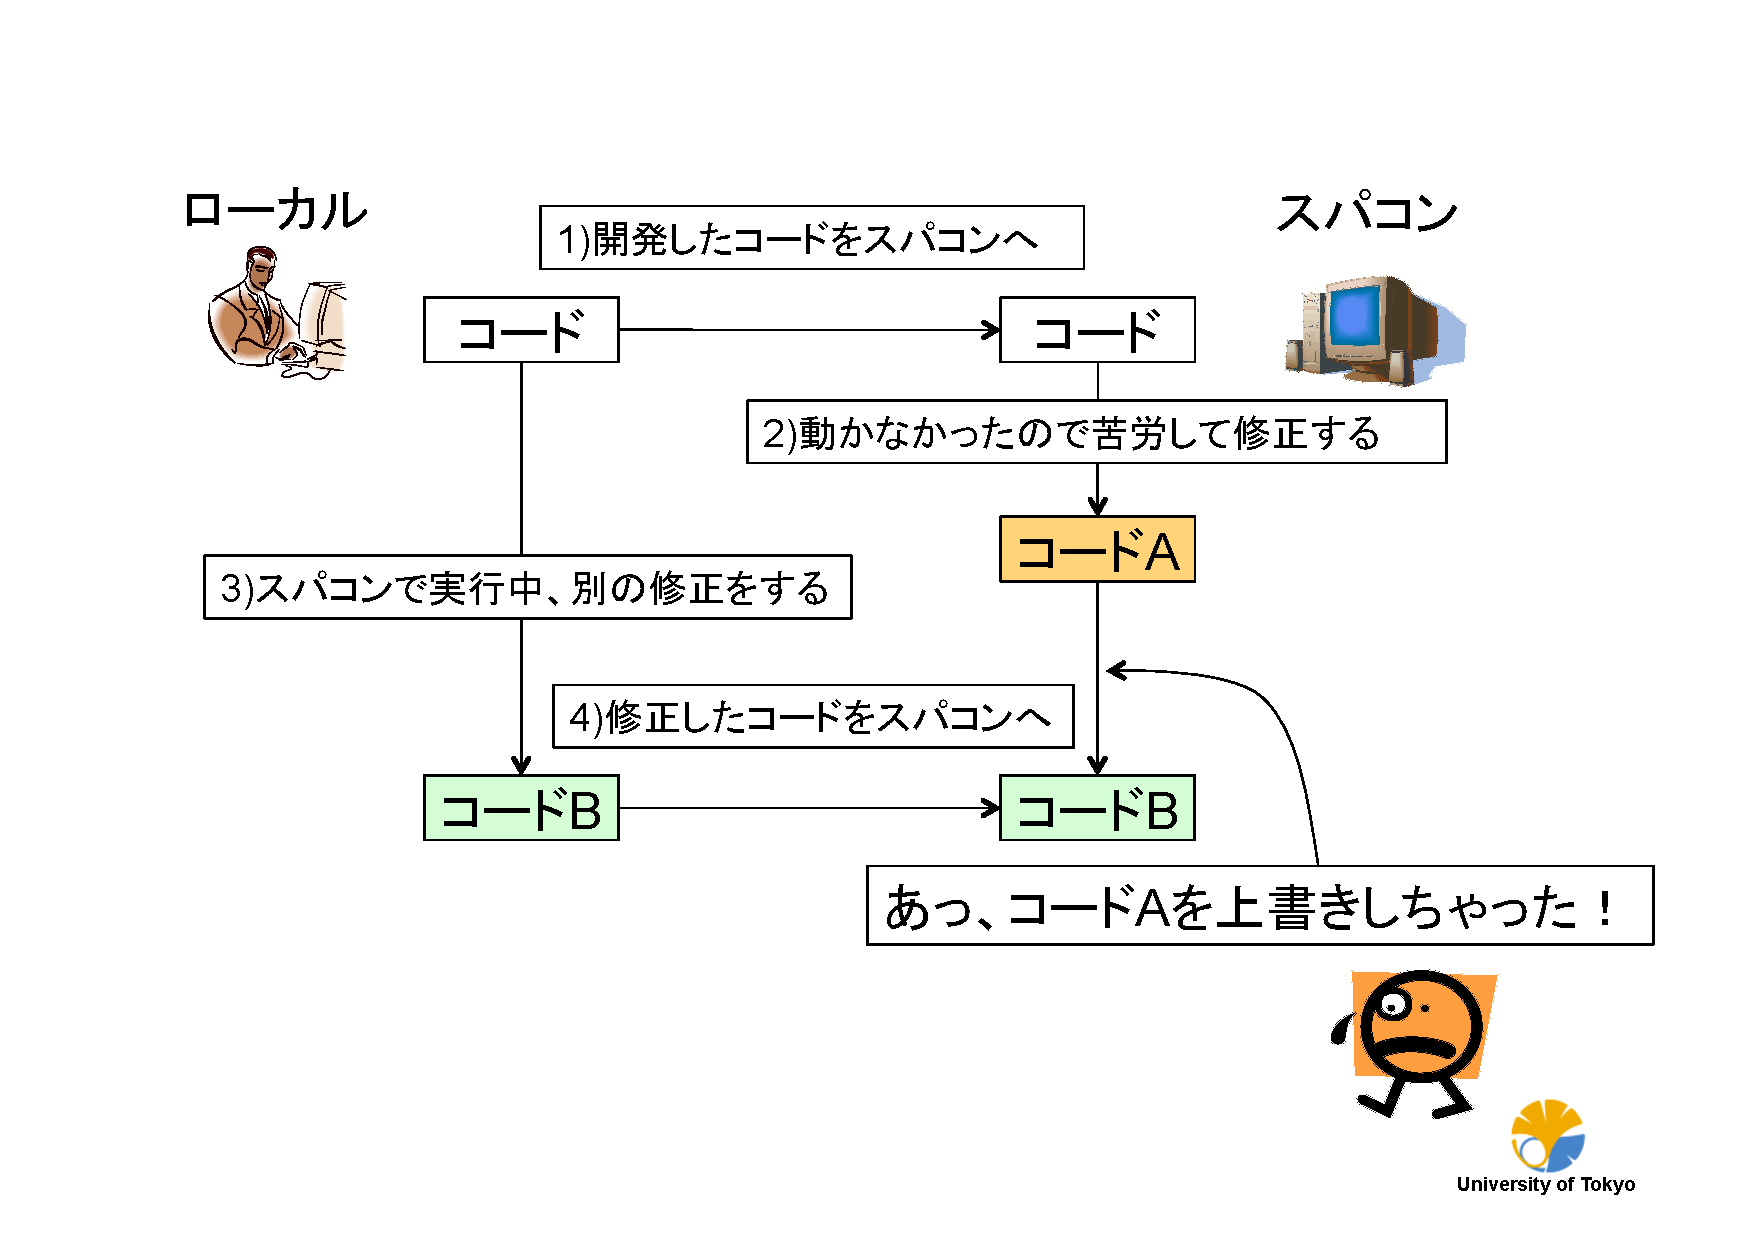
\includegraphics[height=0.88\textheight]{pattern-1.pdf}
  \end{center}
\end{frame}

\begin{frame}
  \frametitle{バージョン管理している場合}
  \begin{center}
    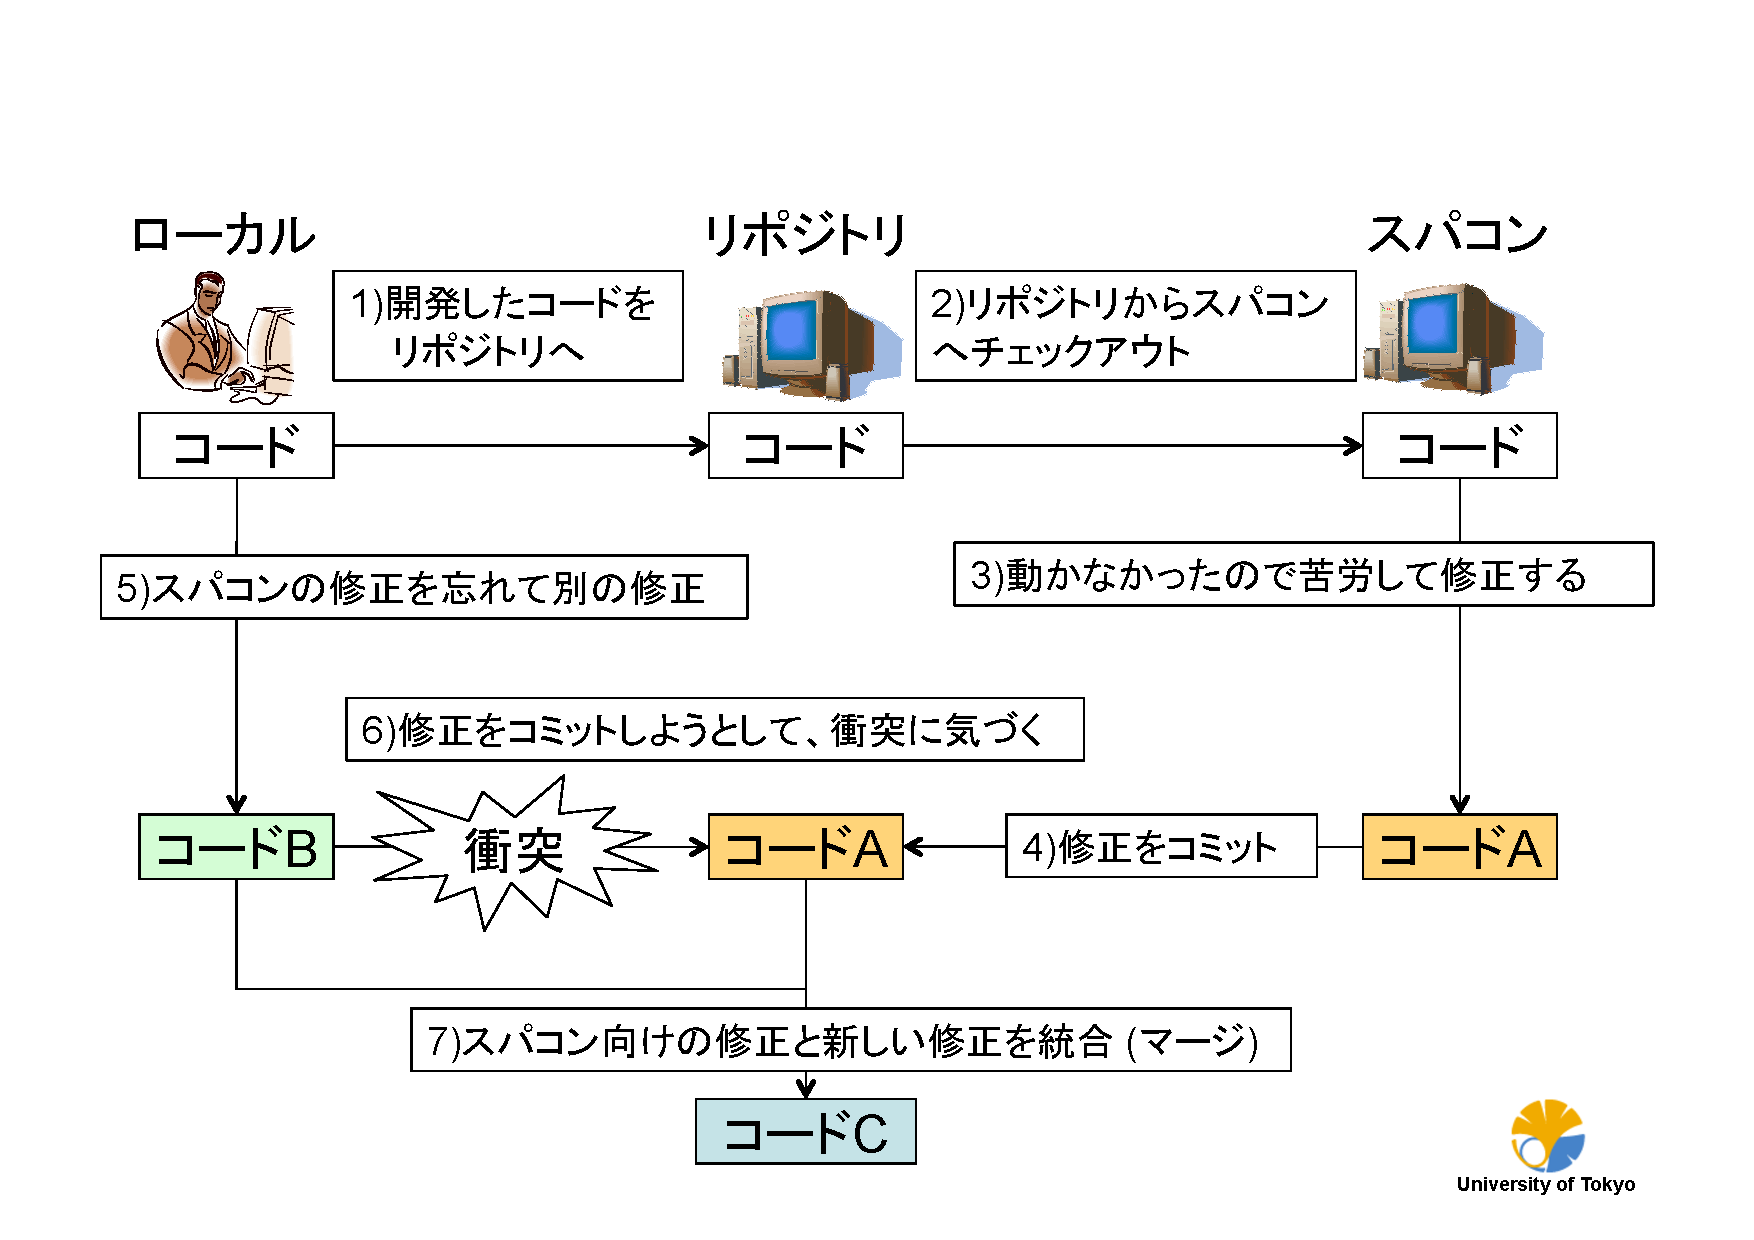
\includegraphics[height=0.78\textheight]{pattern-2.pdf}
  \end{center}
\end{frame}

\begin{frame}
  \frametitle{主なバージョン管理システム}
  \begin{itemize}
  \item BitKeeper - かつて Linux のカーネルのソース管理に使われていた
  \item CVS (Concurrent Versions System) - ネットワークでの利用を考慮とした初めてのバージョン管理システム。以前はよく使われていた
  \item Git - 現在 Linux の開発に使われている。分散型リポジトリ
  \item Mercurial - Git のライバル。分散型リポジトリ
  \item SCCS (Source Code Control System) - 70年代にベル研で開発された世界初のバージョン管理システム。現在は使われない
  \item Subversion - CVSの改良版として開発された。現在最もポピュラー? Mac OS X や多くの Linux には最初からインストールされている
  \end{itemize}
\end{frame}

\begin{frame}
  \frametitle{バージョン管理システムの欠点(面倒な点)}
  \begin{itemize}
  \item 修正前に最新の状態にアップデートしなければならない \\
   ⇒ 慣れると習慣になります
  \item 全ての修正を「コミット」しなければならない \\
    ⇒ 慣れると習慣になります
  \item 衝突(コンフリクト)が発生した時に対処しなければならない \\
    ⇒ 衝突に気づかずに修正してしまうほうが怖いです
  \item サーバのセットアップが面倒くさい \\
    ⇒ まずはホスティングサービス(github, sourceforge, bitbucket)を試してみましょう \\
    ⇒ まわりにいるプロ(?)に相談しましょう \\[.5em]
  \item バージョン管理システムを使うと作業効率が倍以上になる \\
    ⇒ {\color{red} 使わないと人生を半分損する}
  \end{itemize}
\end{frame}

\section{gitの基礎}

\begin{frame}
  \frametitle{gitの基礎}
  \begin{itemize}
  \item 「いつやるの? git入門」ページ28--34, 55, 58--110 \\
    \url{http://www.slideshare.net/matsukaz/git-17499005}
  \end{itemize}
\end{frame}

\begin{frame}[t,fragile]
  \frametitle{実習: gitの基礎(1)}
  \begin{itemize}
  \item ユーザ名などの設定(ログなどに使用される)
\begin{lstlisting}
$ git config --global user.name 'XXXX YYYY'
$ git config --global user.email xxx@yyy.zz
\end{lstlisting}
  \item 作業用ディレクトリとgitリポジトリの作成
\begin{lstlisting}
$ mkdir myproject
$ cd myproject
$ git init
Initialized empty Git repository in /home/xxx/myproject/.git/
$ ls -a
.	..	.git
\end{lstlisting}
  全ての履歴情報は .git に保存される。けっして .git を消さないように!
  \end{itemize}
\end{frame}

\begin{frame}[t,fragile]
  \frametitle{実習: gitの基礎(2)}
  \begin{itemize}
  \item ファイルの作成 \& 管理対象に追加(ステージング)
\begin{lstlisting}
$ vi readme.txt
$ git add readme.txt
$ git status
# On branch master
#
# Initial commit
#
# Changes to be committed:
#   (use "git rm --cached <file>..." to unstage)
#
#	new file:   readme.txt
#
\end{lstlisting}
  \end{itemize}
\end{frame}

\begin{frame}[t,fragile]
  \frametitle{実習: gitの基礎(3)}
  \begin{itemize}
  \item リポジトリに登録(コミット)
\begin{lstlisting}
$ git commit -m 'Initial commit'
[master (root-commit) 5714b10] Initial commit
 0 files changed
 create mode 100644 readme.txt
$ git status
# On branch master
nothing to commit (working directory clean)
\end{lstlisting}
  メッセージ中の``5714b10''がコミットID(の最初の何文字か)
  \end{itemize}
\end{frame}

\begin{frame}[t,fragile]
  \frametitle{実習: gitの基礎(4)}
  \begin{itemize}
  \item ファイルを編集
\begin{lstlisting}
$ vi readme.txt
\end{lstlisting}
  \item 差分を見てみる
\begin{lstlisting}
$ git diff
diff --git a/readme.txt b/readme.txt
index eaf543d..c337c4e 100644
--- a/readme.txt
+++ b/readme.txt
@@ -1 +1,2 @@
 Example of readme file.
+Added a new line.
\end{lstlisting}
  \end{itemize}
\end{frame}

\begin{frame}[t,fragile]
  \frametitle{実習: gitの基礎(5)}
  \begin{itemize}
  \item ステータスを確認
\begin{lstlisting}
$ git status
# On branch master
# Changes not staged for commit:
#   (use "git add <file>..." to update what will be committed)
#   (use "git checkout -- <file>..." to discard changes in working directory)
#
#	modified:   readme.txt
#
no changes added to commit (use "git add" and/or "git commit -a")
\end{lstlisting}
  \end{itemize}
\end{frame}

\begin{frame}[t,fragile]
  \frametitle{実習: gitの基礎(6)}
  \begin{itemize}
  \item ステージング、コミット
\begin{lstlisting}
$ git add readme.txt
$ git commit -m 'Added one line.'
[master c498a65] Added one line.
 1 file changed, 1 insertion(+)
\end{lstlisting}
  \item ログの確認
\begin{lstlisting}
$ git log
commit c498a65ae0a267c206ab1e89fbdb6cfc31d56f2f
Author: Synge Todo <wistaria@issp.u-tokyo.ac.jp>
Date:   Wed Aug 11 22:37:03 2013 +0900

    Added one line.
...
\end{lstlisting}
  \end{itemize}
\end{frame}

\begin{frame}[t,fragile]
  \frametitle{実習: gitの基礎(7)}
  \begin{itemize}
  \item 新しいファイルの作成、ステージング、コミット
\begin{lstlisting}
$ vi hello.txt
$ git add hello.txt
$ git commit -m 'Created hello.txt'
\end{lstlisting}
  \item サブディレクトリの下にファイルを作成
\begin{lstlisting}
$ mkdir src
$ vi src/myprog.f
$ git add src/myprog.f
$ git commit -m 'Initial version of myprog.f'
\end{lstlisting}
  \item ファイルの削除、移動、コミット間の差分
  \end{itemize}
\end{frame}

\section{ブランチとマージ}

\begin{frame}
  \frametitle{ブランチとマージ}
  \begin{itemize}
  \item 「いつやるの? git入門」ページ112--152 \\
    \url{http://www.slideshare.net/matsukaz/git-17499005}
  \item 「こわくないGit」ページ6--78 \\
    \url{http://www.slideshare.net/kotas/git-15276118}
  \end{itemize}
\end{frame}

\begin{frame}[t,fragile]
  \frametitle{実習: ブランチとマージ(1)}
  \begin{itemize}
  \item develop ブランチの作成
\begin{lstlisting}
$ cd myproject
$ git branch develop
$ git checkout develop
Switched to branch 'develop'
$ git branch
* develop
  master
\end{lstlisting}
  \item develop ブランチに doc.txt を作成
\begin{lstlisting}
$ vi doc.txt
$ git add doc.txt
$ git commit -m 'Created documentation'
[develop 9b5f323] Created documentation
 1 file changed, 1 insertion(+)
 create mode 100644 doc.txt
\end{lstlisting}
  \end{itemize}
\end{frame}

\begin{frame}[t,fragile]
  \frametitle{実習: ブランチとマージ(2)}
  \begin{itemize}
  \item masterブランチに戻ってみる
\begin{lstlisting}
$ git checkout master
$ ls
hello.txt	readme.txt	src
\end{lstlisting}
doc.txt がなくなっていることに注意 \\[.5em]
  \item もう一度、developブランチに切り替え
\begin{lstlisting}
$ git checkout develop
$ ls
doc.txt		hello.txt	readme.txt	src
\end{lstlisting}
  \end{itemize}
\end{frame}

\begin{frame}[t,fragile]
  \frametitle{実習: ブランチとマージ(3)}
  \begin{itemize}
  \item masterブランチでファイルを編集、コミット
\begin{lstlisting}
$ git checkout master
$ vi hello.txt
$ git add hello.txt
$ git commit -m 'Modified hello.txt'
\end{lstlisting}
この時点で master と develop が枝分かれ! \\[.5em]
  \item developブランチをmasterブランチにマージ
\begin{lstlisting}
$ git merge develop
Merge made by the 'recursive' strategy.
 doc.txt |    1 +
 1 file changed, 1 insertion(+)
 create mode 100644 doc.txt
\end{lstlisting}
  \end{itemize}
\end{frame}

\begin{frame}[t,fragile]
  \frametitle{実習: ブランチとマージ(4)}
  \begin{itemize}
  \item コミットグラフ(の一部)を表示
\begin{lstlisting}
$ git log --graph
...
\end{lstlisting}
github (後述)を使っている場合には、web上でコミットグラフを見ることができる
  \end{itemize}
\end{frame}

\begin{frame}[t,fragile]
  \frametitle{実習: ブランチとマージ(5)}
  \begin{itemize}
  \item 今度はコンフリクトが起こるような修正を行ってみる
\begin{lstlisting}
$ git checkout develop
$ vi hello.txt  # 先程と同じ場所を違う文字列に修正
$ git add hello.txt
$ git commit -m 'Modified hello.txt differently'
\end{lstlisting}
  \item マージしようとすると失敗する!
\begin{lstlisting}
$ git checkout master
Switched to branch 'master'
$ git merge develop
Auto-merging hello.txt
CONFLICT (content): Merge conflict in hello.txt
Automatic merge failed; fix conflicts and then commit the result.
\end{lstlisting}
  \end{itemize}
\end{frame}

\begin{frame}[t,fragile]
  \frametitle{実習: ブランチとマージ(6)}
  \begin{itemize}
  \item hello.txtの中を見るとコンフリクトした箇所がわかる
\begin{lstlisting}
$ cat hello.txt
<<<<<<< HEAD
Hello, CMSI
=======
Hello, MateriApps
>>>>>>> develop
\end{lstlisting}
'\verb+<<<<<<<+'と'\verb+>>>>>>>+'の間の領域がコンフリクト \\[.5em]
  \item ファイルを編集してコンフリクトを解消、コミット
\begin{lstlisting}
$ vi hello.txt
$ cat hello.txt
Hello, MateriApps
$ git add hello.txt
$ git commit -m 'Merge branch develop'
\end{lstlisting}
  \end{itemize}
\end{frame}

\section{リモートリポジトリとの連携}

\begin{frame}
  \frametitle{リモートリポジトリとの連携}
  \begin{itemize}
  \item 「いつやるの? git入門」ページ154--193 \\
    \url{http://www.slideshare.net/matsukaz/git-17499005}
  \end{itemize}
\end{frame}

\begin{frame}
  \frametitle{実習: リモートリポジトリとの連携}
  \begin{itemize}
  \item githubのリポジトリ
  \item (時間があれば)「Git道場 技 本日の課題、 テクニックの解説」 \\
    \url{https://speakerdeck.com/ogawa/git} に従って演習
  \end{itemize}
\end{frame}

\begin{frame}
  \frametitle{バージョン管理システムを使う上での注意点}
  \begin{itemize}
  \item gitが管理している領域からファイルを持ちだして編集してはいけない。
  \item 大きなバイナリファイル(PDF, DOC, tar.gzなど)をgitで管理しない。
  \end{itemize}
\end{frame}

\section{githubを用いたオープンソース・ソフトウェアの開発・公開}

\begin{frame}
  \frametitle{「公開ソフト」が備えているべきもの}
  \begin{itemize}
  \item マニュアル
  \item チュートリアル
  \item ライセンス
  \item ビルドシステム・インストーラー
    \begin{itemize}
    \item ソースコード配布 \\
      Linuxで一般的。ソースと一緒にビルド環境(Makefile, CMake, configure スクリプト)を配布
    \item バイナリ配布 \\
      Windowsで一般的。バイナリインストーラ形式で配布
    \end{itemize}
  \item ユーザフレンドリな操作環境(GUIなど)
  \item ユーザサポート体制
  \end{itemize}
\end{frame}

\begin{frame}
  \frametitle{ビルドシステム: CMake}
  \begin{itemize}
    \setlength{\itemsep}{1em}
  \item Makefileを生成するためのユーティリティー (configureスクリプトに対応)
    \begin{itemize}
    \item Windows の Visual C++ 用ソリューションファイル, Mac OS X の Xcode 用プロジェクトファイルの生成も可能
    \end{itemize}
  \item 設定は CMakeLists.txt に記述する
  \item テスト(CTest)やバイナリインストーラ作成(CPack)の機能もある
  \item ファイルの依存関係の自動検出
  \end{itemize}
\end{frame}

\begin{frame}
  \frametitle{オープンソース・ソフトウェア開発の流れ (例)}
  \begin{itemize}
    %\setlength{\itemsep}{1em}
  \item github にリポジトリを作成
  \item 開発
    \begin{itemize}
    \item ソースコード
    \item ビルドシステム
    \item ドキュメント類
    \item テスト
    \end{itemize}
  \item バージョン番号を割り当て
  \item 公開
    \begin{itemize}
    \item 配布物の作成 (tar.gz, インストーラー)
    \item 配布物のアップロード (sourceforge)
    \item アナウンス
    \end{itemize}
  \item 次期バージョンの開発へ
  \end{itemize}
\end{frame}

\section{その他}

\begin{frame}
  \frametitle{その他の話題}
  \begin{itemize}
    \setlength{\itemsep}{1em}
  \item MateriAppsとMateriApps Liveの紹介
  \item A successful Git branching model (ブランチの上手な使い方) \url{http://keijinsonyaban.blogspot.jp/2010/10/successful-git-branching-model.html}
  \item Gitをボトムアップから理解する (gitの中で何が起こっているのかを知りたい人向け) 
    \url{http://keijinsonyaban.blogspot.jp/2011/05/git.html}
  \end{itemize}
\end{frame}

\end{document}
